\section{Conclusion}
\label{sec:conclusion}
This work has presented a generic approach for multi-robot exploration and mapping using RGB-D cameras as main sensor. The problem has been tackled by considering its sub-challenges, namely SLAM and point cloud handling, exploration strategy and path planning.

\begin{figure}[H]
  \begin{center}
    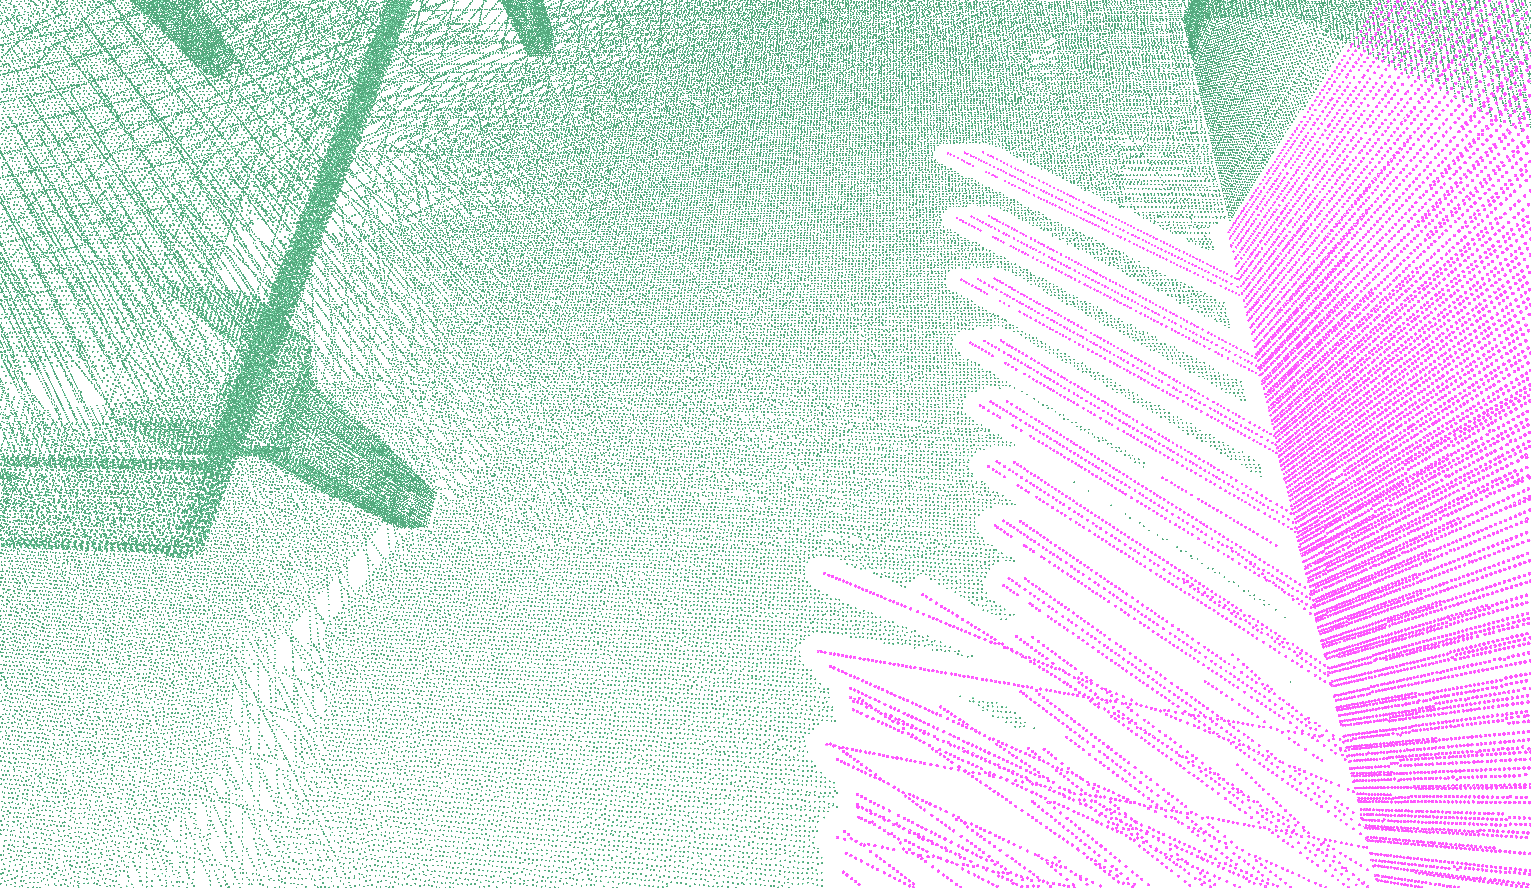
\includegraphics[width=0.49\textwidth]{img/example.png}
  \end{center}
  \caption[]{
    \textbf{Particular on points selection} 
  }
  \label{fig:example}
\end{figure}


Overall, the proposed framework is capable of achieving an accurate mapping, leveraging the capabilities of the RTAB-Map software and point cloud merging algorithms. At the same time, the proposed strategies for exploration and navigation guarantee efficiency and safety in obstacle avoidance.

Future work will focus on testing the system with a larger number of agents, potentially deploying the software on real robots. Any knowledge a-priori of the environment, like QR codes, could be used as loop closure triggers, relieving the software from identifying closures from visual features. In the exploration task, more complex reward functions can be defined and new assignment strategies can be tested. 


%Implementation of logic based on qr codes:} the qr codes could be used in a way: on one side they could be used as loop closure triggers, on the second side a logic of navigation could be developed. For the first usage, the qr codes could be put in sections where bottlenecks occur and it is guaranteed that the robots will all visit that section, therefore letting them now to have a best attempt in loop closure in that specific region. For the second usage, this placement could be used as "direction sign" if any knowledge of the map is known a-priori, leading to a better organization of the robots and locations covered

% Still relatively computationally expensive, but mostly because we deploy RTAB-Map for every robot and the amount of data to be computed in real time comprises all the point clouds generated. Different approaches can optimize this aspect, like density of the point cloud and area mapped at each iteration, but these come at a cost of quality and completeness of the map.  
%New reward functions and assignment, non greedy magari.